\documentclass[a4paper,12pt]{article}
\usepackage{graphicx} 
\usepackage{hyperref}
\usepackage{float}
\usepackage{amsmath}
\usepackage{amsfonts}
% \usepackage{enumitem}

% \begin{figure}[H]
%     \centering
%     \includegraphics[width=0.7\textwidth]{filename.png}
%     \caption{Your figure caption here.}
%     \label{fig:yourlabel}
% \end{figure}

\begin{document}

\title{Assignment 2 - Theoretical Questions}
\author{Mohammad Hossein Basouli}
\date{\today}
\maketitle

\section*{Question 1}
\textbf{Correlation} and \textbf{causality} are two different concepts in decission making, often confused with each other. \textbf{Correlation} only specifies whether if there is a relationship
between the two variables, where \textbf{causality} talks about the effect that a cause happens to make. The \textbf{correlation} could be even meaningless, e.g. increase of \textit{divorce} along with increase
of \textit{house price}. Also the \textbf{correlation} (if it actually is a meaningful \textbf{correlation} and not just a coincidence!) doesn't specify which of the variables causes the other or if there is a 
third variable in between, that is causing these two variables. \\

\noindent \textbf{Example}: assume that the number of sunburns in a town recorded for a month has a positive \textbf{correlation} with number of ice creams eaten. This obviously is a meaningful \textbf{correlation}, 
because we expect these two to increase together; but we can't say that number of ice creams eaten causes the number of sunburns or the other way around because the sunny weather is actually the cause of these two to increase together. 

\section*{Question 2}
\textit{(I couldn't label the items with alphabets so we go with numbers.)}

\begin{enumerate}
    \item \textbf{Issues of the raw data}:
    \begin{itemize}
        \item \textbf{Data incompleteness}
        \item \textbf{Data noisyness}
        \item \textbf{Data inconsistency}
    \end{itemize}
    \item \textbf{Four major tasks in data preprocessing}:
    \begin{itemize}
        \item \textbf{Data Integration}: Gathering the data from multiple sources and integrating them.
        \item \textbf{Data Cleaning}: Detecting and handling missing values, outlies, noisy data, etc.
        \item \textbf{Data Transformation}: Aggregation and Normalization.
        \item \textbf{Data Reduction}: Removing unnecessary features, droping some of the rows, etc.
    \end{itemize}
    \item \textbf{Ways to handle missing values}:
    \begin{itemize}
        \item \textbf{Dropping the rows}
        \item \textbf{Imputation}:
        \begin{itemize}
            \item Filling in the missing values by mean or
            \item By a constant.
            \item Mean of the class that the data belongs to.
        \end{itemize}
    \end{itemize}
\end{enumerate}

\section*{Question 3}
Binning could be used to smooth the noise in the data, it moves the data points that are in the same bin (or a close interval) towards the mean, median or the boundary of the bin. 
\textbf{Example}: Consider the data points [5, 6, 8, 100, 7, 6, 5]. We first sort the data and then put them into the bins of size 3. Here is how it would look like. \\ 
Bin 1: [5, 6, 8] $\rightarrow$ Mean = 6.33 $\rightarrow$ Smoothed bin: [6.33, 6.33, 6.33] \\ 
Bin 2: [100, 7, 6] $\rightarrow$ Mean = 37.67 $\rightarrow$ Smoothed bin: [37.67, 37.67, 37.67]  

\section*{Question 4}
\begin{enumerate}
    \item \textbf{Importance of data quality in EDA and common issues such as outliers and data inconsistency}:
    \begin{itemize}
        \item \textbf{data quality is important in following aspects}:
        \begin{itemize}
            \item extracting accurate insights from the data analysis.
            \item performance of the model.
        \end{itemize}
        \item \textbf{issues with outliers}:
        \begin{itemize}
            \item could affect statistical measures badly. (data skewness, mean, standard deviation, etc.)
            \item causes misinterpretations from the visulization. (misinterpretation of the distribution of the data, etc.)
        \end{itemize}
        \item \textbf{Issues with inconsistencies}:
        \begin{itemize}
            \item could lead to misunderstanding of the data. (Consider having different representations of a single category in our data; like having [NA, New York, na, ...] to represent
            a single city. They are all the same city but are represented as different values.)
            \item leading to difficulty in the analysis.
        \end{itemize}
    \end{itemize}
    \item A scenario where data quality issues lead to misleading conclusions in a real-world analysis:
    Assume that we have a dataset of the cars insured by an insurance company, and the dataset has been recorded by multiple different operators who don't agree to follow a similar convention
    while recording car models. Consider the car model \textit{Kia Pride CD5 (1999)}, one could record it as \textit{1999 Kia Pride}, the other one as \textit{Pride 5 doors}, and so on. This would lead us to have many different representations of a single model 
    of car, increasing the complexity when we want to put up car model as a feature in our model our data analysis.
    \item \textbf{EDA techniques for identfying and addressing the data quality issues}:
    \begin{itemize}
        \item \textbf{outliers issues}: with the help of visulization, smoothing, etc. we can get rid of outliers in our dataset. 
        \item \textbf{inconsistency issues}: database integration and management techniques could help to get rid of inconsistency issues. 
    \end{itemize}
\end{enumerate}

\section*{Question 5}
\begin{itemize}
    \item \textbf{Min-Max Normalization}: 
    \( x' = \frac{x - \min(x)}{\max(x) - \min(x)} \) 
    it begin the data in the range [0, 1], and also keeps the original distribution of the data.
    \item \textbf{Standardization}:
    \( x' = \frac{x - \mu}{\sigma} \) 
    this would transform a normal distribution with mean $\mu$ and std $\sigma$ to z distribution. 
    \item \textbf{Robust Scaling}:
    \( x' = \frac{x - \text{median}(x)}{\text{IQR}(x)} \)
    this ia a bit more less sensitive to outliers compared to Min-Max Normalization
\end{itemize}

\section*{Question 6}
The goal of \textbf{data reduction} is to reduce the data in volume while still maintaining critical information about the data. Different techniques used in this approach are as follows.
\begin{itemize}
    \item \textbf{Data Cube Aggregation}: aggregation of multiple rows to produce a single new row, representing the other information in those rows.
    \item \textbf{Dimentionality Reduction}: removing highly correlated columns in order to simplify the dataset.
    \item \textbf{Numerosity Reduction}: using clustering to divide the dataset into multiple different clusters and then selecting only a few data points in those clusters (it could be just the mean of that cluster) to represent the other data points in the cluster.
\end{itemize}

\section*{Question 7}
\begin{enumerate}
    \item Because visulization is one of the most natural, simplest and most powerful ways to convey ideas and insight to others. An specfic concept gets undertood so much easier through visulization most of time.
    \item Consider this example: Figure~\ref{fig:Figure_1} shows an uncolorized, unmarked useless plot showing the the line plot of hire, promotion and transfers in a company on different 
    times; It doesn't give us a whole lot of details about these variables such as do we have a special pattern in our hires over time, etc. . But Figure~\ref{fig:Figure_2} shows a well 
    guided plot, which essentially contains within different stories about the data, what months represent the peaks in our hires ? is there a pattern such as what months in a year are 
    having a significantly higher hires? This plot captures the answer to all of this information. e.g. it tells us that the first month in each quarter of the year has a peak in the hires compared
    to the other months.
    
    \begin{figure}[H]
        \centering
        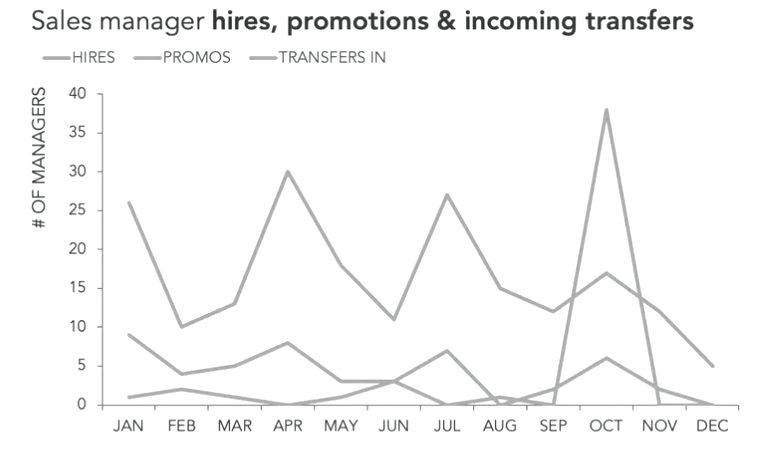
\includegraphics[width=0.7\textwidth]{traditional_visulization.png}
        \caption{Traditional Visualization}
        \label{fig:Figure_1}
    \end{figure}

    \begin{figure}[H]
        \centering
        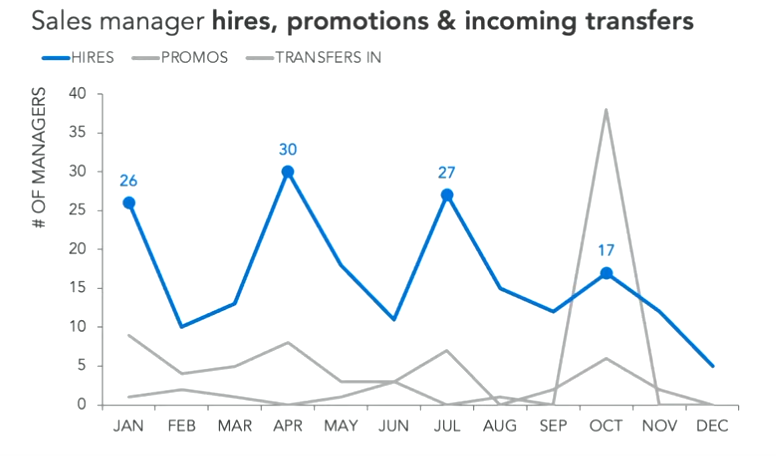
\includegraphics[width=0.7\textwidth]{storytelling.png}
        \caption{Visulization with Storytelling}
        \label{fig:Figure_2}
    \end{figure}
    
    \item \textbf{What elements transform a chart into a compelling story telling}:
    \begin{itemize}
        \item Annonations 
        \item Highlights and colors
        \item Well chosen and oriented labels for axis
        \item Descriptive title
    \end{itemize}
\end{enumerate}

\section*{Question 8}
\begin{enumerate}
    \item \textbf{factors that determine the best type of chart to use for a dataset}:
    \begin{itemize}
        \item data type of the variables. (Whether they are ordinal/nominal categorical or numerical)
        \item our needs and the questions we have about the dataset. (e.g. if we want to see whether if there is a monotonic relationship between two variables, we can use scatter plot of these two variables.)
        \item number of variables
        \item data density and size
    \end{itemize}
    \item \textbf{importance of distribution charts in EDA}:
    \begin{itemize}
        \item detecting outliers and anomalies.
        \item getting insight about the original distribution of the data.
        \item identifying relationship between variables.
        \item helps in forming hypothesis about the data.
    \end{itemize}
    \item \textbf{How a heatmap of a correlation matrix can help identify patterns in a multivariate dataset:} A heatmap of the correlation matrix visually represents the pairwise correlations between variables using color intensity. More intense or darker squares typically indicate stronger positive or negative correlations between the corresponding variables. This makes it easier to detect linear relationships, clusters of related variables, or potential multicollinearity at a glance.
\end{enumerate}

\section*{Question 9}
\textbf{pie chart}
\begin{itemize}
    \item \textbf{insight}: Compares the percentages of data in each of the different category levels.
    \item \textbf{suitable data types}: categorical
\end{itemize}

\textbf{line chart}
\begin{itemize}
    \item \textbf{insight}: How the trend of the data might look like as the time passes.
    \item \textbf{suitable data types}: two variable - numerical and numerical 
\end{itemize}

\textbf{bar chart}
\begin{itemize}
    \item \textbf{insight}: How much data in each of the category levels resides and how the overal distribution of the variables looks like.
    \item \textbf{suitable data types}: one variable - categorical
\end{itemize}










\end{document}